\documentclass[11pt]{article}

\input preamble

%\newdimen\tlx
%\newdimen\tlx
%\newdimen\brx
%\newdimen\bry

\title{BDBags and Minids:\\A Framework for FAIR Big Data Science}
\author{}
\date{}

\begin{document}
\maketitle


\section{Introduction}

Big data from high throughput experiments and other sources create exciting new opportunities for biomedical discovery. 
They also present considerable challenges %for researchers and indeed for the research process, 
due to the difficulties inherent in manipulating large data volumes and capturing the resulting analysis workflows in reproducible forms.
In particular, despite broad acceptance of the need to ensure that data are
Findable, Accessible, Interoperable, and Reusable (FAIR)~\cite{wilkinson16},
many big data languish unfindable, inaccessible, non-interoperable, and thus non-reusable.

In response, the NIH BD2K Big Data for Discovery Science (BDDS) center~\cite{toga15}
has developed two powerful new constructs that simplify the realization of FAIRness in 
complex big data applications: Big Data Bags (BDBags) for data exchange and 
minimal identifiers (Minids) as persistent identifiers for intermediate data products.
Together, and in conjunction with other tools developed by BDDS team members and partners,
these constructs \textbf{allow even the largest biomedical data to be captured, exchanged, and shared 
in reusable forms that are accessible via persistent identifiers}. 
The result, as we show in a variety of applications, is that big data becomes easy to find, access, integrate, and (re)use. 
%Modern tools can be used to automate routine but complex tasks, capture analysis algorithms in understandable and reusable forms, and harness fast networks and powerful cloud computers to process data rapidly without sacrificing usability or reproducibility. 

\vspace{2ex}

\noindent\shadowbox{%
    \parbox{0.985\textwidth}{%
The BDDS contributions to FAIR big data science described in this document span four areas:
\begin{enumerate}
\itemsep0em 
\item
The \textbf{BDBag exchange format and Minid identifier} for the exchange of big scientific data,
with comprehensive support for
``holey" bags (i.e., bags that contain references to remote data)
and for associating descriptions of bag contents in the form of a Research Object~\cite{bechhofer2013linked}.

\item
High-quality \textbf{open source implementations} of a comprehensive set of  
command line tools, Python APIs, and graphical user interface for manipulating BDBags and Minids.
%along with associated file references and RO description,
%for resolving files that are represented via remote references, for validating
%bags, for creating bags of bags, and other purposes.

\item
\textbf{Integration} of BDBag and Minid mechanisms with a range of other tools, 
such as Globus and Galaxy 
to provide end-to-end solutions to the problem of organizing and sharing big data. 

\item
Compelling \textbf{example applications} that demonstrate the value of BDBag and Minid capabilities,
such as an ENCODE portal, transcription factor binding site analysis~\cite{madduri2018reproducible}, and
Peptide Atlas.
\end{enumerate}

\vspace{-1ex}
}
}

\section{BDBags and Minids: Why, What, and How}

%\vspace{1ex}
%
%\noindent
%\textbf{The problem.}
Big data science requires mechanisms for describing, referring to,
and exchanging large  and complex datasets that may comprise many directories and files (elements).
The following five requirements are key:
%Five key requirements are~\cite{chard16}:
\begin{enumerate}
\itemsep0em 
\item
\textbf{Enumeration}: Explicit enumeration of a dataset's elements, so that
subsequent additions or deletions can be detected.
\item
\textbf{Fixity}: Enable verification of dataset contents, 
so that data consumers can detect errors in data transmission or modifications to data elements.
\item
\textbf{Description}: Provide interoperable methods for tracking the attributes (metadata) and origins (provenance) of dataset contents; 
\item
\textbf{Distribution}: Allow a dataset to contain elements from more than one location.
\item
\textbf{Identification}: Provide a reliable and concise way of referring to datasets for purposes of collaboration, publication, and citation.
\end{enumerate}

%\begin{figure}
%\begin{tabbing}
%aa\=aa\=aa\=aaaaaaaaaaaaaaaaaaaaaaaa\=aa\=aa\=\kill
%{\tt \small examplebag/} \>\>\>\> Top level name\\
%\> \texttt{\textbf{\small bag-info.txt}} \>\>\>  Metadata for the bag\\
%\> {\tt \small bagit.txt} \>\>\>  BagIt version and encoding information \\
%\>  {\tt \small data/} \>\>\>  The BDBag's contents:\\
%\>\> {\tt \small mydirectory/} \>\>\> User directory \\
%\>\>\>  {\tt \small file1} \>\>\>A first user file \\
%\>\>\>  {\tt \small file2}\>\>\>  A second user file \\
%\>  \texttt{\textbf{\small fetch.txt}} \>\>\>  How to fetch missing elements \\
%\>  {\tt \small manifest-md5.txt} \>\>\> MD5 checksums for data files\\
%\>  {\tt \small manifest-sha256.txt} \>\>\> SHA checksums for data files\\
%\>  {\tt \small metadata/} \>\>\>  Tag directory for Research Object metadata\\
%\>\>  \texttt{\textbf{\small manifest.json}}\>\> \> Research Object metadata as JSON-LD\\
%\>  \texttt{\textbf{\small tagmanifest-md5.txt}} \>\>\>  MD5 checksum for tags\\
%\>  \texttt{\textbf{\small tagmanifest-sha256.txt}} \>\>\> SHA checksum for tags
%\end{tabbing}
%\caption{An example BDBag, with contents in the \texttt{data} folder, 
%description in the \texttt{metadata} folder, and other elements providing data required to
%fetch remote elements (\texttt{fetch.txt}) and validate its components.\label{fig:2}}
%\end{figure}

Surprisingly, we determined early in BDDS that no existing technology addressed these requirements.
Thus we made the development and demonstration of suitable mechanisms a major focus of the BDDS center.
As part of this work, we developed two important new technologies, BDBags and Minids, each
defined in terms of existing standards and
implemented in ways that permit easy integration into a wide variety of
applications and workflows, without deployment of complex software on researcher computers~\cite{chard16}.

%\begin{enumerate}
%\item
%the Big Data Bag (\textbf{BDBag}) exchange format and associated tools address the \emph{enumeration}, \emph{fixity}, \emph{description}, and \emph{distribution} requirements and
%provide a robust mechanism for exchanging large and complex data collections; and 
%%the Big Data Bag (\textbf{BDBag}) for defining a dataset and its contents by enumerating and describing its elements, 
%%regardless of their location (addressing \emph{enumeration}, \emph{fixity}, \emph{description}, \emph{distribution});
%%the Research Object (RO)~\cite{bechhofer2013linked} to characterize a dataset and its contents with arbitrary levels of detail, regardless of their location (description);
%and
%\item
%the \textbf{Minid} identifier and associated tools address the \emph{identify} and \emph{fixity} requirements
%and provide mechanisms for uniquely identifying a dataset and, if desired, its constituent elements, 
%regardless of their location.
%\end{enumerate}

\subsection{Big Data Bags for exchange of large and complex data}

The Big Data Bag (\textbf{BDBag}) exchange format and associated tools address the \emph{enumeration}, \emph{fixity}, \emph{description}, and \emph{distribution} requirements given above.
They provide a robust mechanism for exchanging large and complex data collections.

In defining the BDBag exchange format, 
we build on and extend an Internet Engineering Task Force (IETF) specification, BagIt~\cite{Kunze2015}.
A dataset's contents are captured as
directories and files contained within a \texttt{data} directory,
with other elements providing checksum and metadata information (e.g., type and provenance)
required to verify and interpret the data.
%Research Object~\cite{bechhofer2013linked} mechanisms can be used to specify
%of the type and provenance of BDBag contents
References to remotely accessible data can be included in a \texttt{fetch.txt} file. 
%with the information required to retrieve those data provided in a \texttt{fetch.txt} file as a (URL, LENGTH, FILENAME) triple.  
The ability to reference remote data allows for the concise specification of large datasets, and
also allows the definition of data collections that specific individuals may not have immediate permission to access, 
as when access to data elements is restricted by data use agreements.

We then developed a comprehensive suite of tools for creating BDBags, for
materializing the data in a BDBag in a standard way, for capturing metadata, 
and for verifying contents based on checksums of individual data and metadata items.

\vspace{2ex}

\noindent\shadowbox{%
    \parbox{0.985\textwidth}{%
The BDBag makes it possible to
capture in a concise document a consistent, self-describing, integrity-verifiable description of even
extremely large quantities of data.
A BDBag of just a few hundred bytes may contain references to many terabytes, and 
can be stored, referenced in a paper, and exchanged with other researchers or tools
and then resolved at any point to access the referenced data.
}}

%\begin{figure}
%\centering
%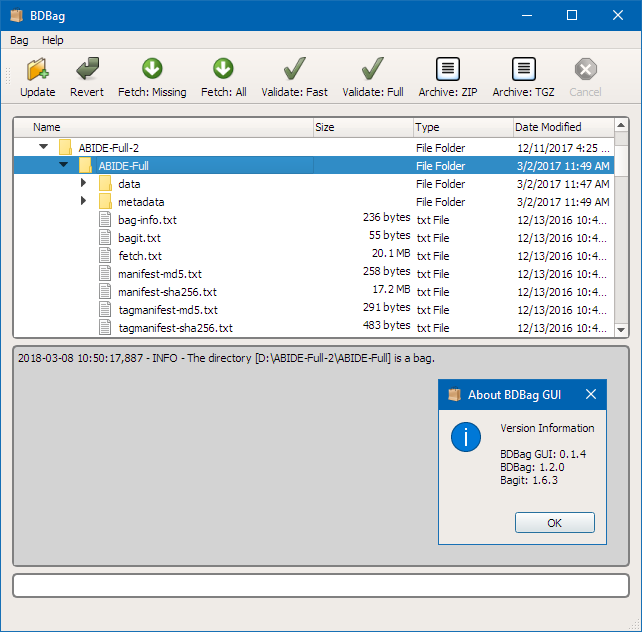
\includegraphics[width=0.8\textwidth]{figs/bdbag_gui_version.png}
%\caption{To give a flavor of the BDBag specification, we show an example of the BDBag GUI application selecting a bag
%representing the ABIDE preprocessed dataset available at \smallurl{https://bd2kcat1.ini.usc.edu/abide/search/}.}
%\end{figure}

%\noindent\fbox{%
%    \parbox{\textwidth}{%
%In summary, our contributions span four areas:
%\begin{enumerate}
%\item
%We designed, and obtained broad community support for, BagIt extensions that allow for big scientific data.
%These extensions include comprehensive support for
%``holey" bags (i.e., bags that contain references to remote data)
%and mechanisms for associating descriptions of bag contents in the form of a Research Object~\cite{bechhofer2013linked}.
%
%\item
%We developed high-quality open source implementations of tools for creating BDBags,
%%along with associated file references and RO description,
%for resolving files that are represented via remote references, for validating
%bags, for creating bags of bags, and other purposes.
%
%\item
%We integrated these mechanisms with a range of other tools, 
%from Minids and Globus to ENCODE and Galaxy 
%to provide an end-to-end solution to the problem of organizing and sharing big data. 
%
%\item
%We developed compelling example applications that demonstrate the value of BDBag capabilities.
%
%\end{enumerate}
%}
%}

%These mechanisms enable the exchange of large, self-describing datasets without copying large amounts of data.
%Indeed, a ``holey'' BDBag that a hundreds of bytes in size can provide a complete description of 



%(a ``holey'' BDBag that contains only references, not data, may be just a few hundreds of bytes in size

%The BDBag specification adopts the \textbf{Research Object} (RO) framework to associate attribution and provenance information, and structured and unstructured annotations describing individual resources, with the data contained in a BDBag.
%A BDBag's metadata directory contains annotations and the RO manifest.json in JSON-LD format~\cite{JSONLD}: see Fig~\ref{fig:2}.

%\begin{figure}
%\centering
%\fbox{\includegraphics[width=0.8\textwidth,trim=0.2in 1.6in 3.2in 0.3in,clip]{figs/LandingPage-new.pdf}}
%\caption{A Minid landing page for a BDBag generated by the \texttt{encode2bag} tool,
%showing the associated metadata, including locations (in this case, just one).\label{fig:3}}
%\end{figure}

\subsection{Minid: A minimal viable identifier}

The minimal viable identifier (\textbf{Minid}) identifier and associated tools address the \emph{identify} and \emph{fixity} requirements
identified above~\cite{chard16}.
%They provide mechanisms for uniquely identifying a dataset and, if desired, its constituent elements, 
%regardless of their location.

We designed the Minid to meet researcher needs
for robustly naming the many datasets that may be created in the course of their work, 
so that they can uniquely reference and locate data,
and share and exchange names (rather than an entire dataset),
while being able to ensure that a dataset's contents are unchanged.
The Digital Object Identifiers (DOIs) that are sometimes used for this purpose
are heavyweight constructs designed for naming resources such as scholarly articles
that are created only rarely.
Minids, by contrast, are lightweight, low-cost identifiers %designed to enable frequent creation;
that can be easily created, resolved, and used in their millions. 

Minids  take the form \texttt{minid:[suffix]}, where  the suffix is a unique sequence of characters
and can be resolved, for example via \texttt{\href{https://n2t.net}{n2t.net}},
so that visiting
\texttt{\href{https://n2t.net/minid:b9j01d}{https://n2t.net/minid:b9j01d}} 
redirects the browser to the landing page for the
object with identifier \texttt{minid:b9j01d}.
Importantly, a Minid can link to more than one location for the referenced data.
%allowing for data replication.
%For example, a Minid may reference 
for example, one copy in the source repository, 
additional copies in different cloud object stores, and another on a local file system.
Because a Minid includes a checksum of the content, 
we can ensure that whatever copy is used, it contains the correct and intended content.
The consumer can then determine which copy of the data is ``best'' for their purpose.
%and the responsibility of the Minid creator to interact with the landing page service to register new copies.
%The GET methods for the landing page support HTTP content negotiation;
%results may be returned in human-readable (HTML) or machine-readable (JSON) form.

As with BDBags, we created the Minid construct via the artful combination of existing and new capabilities.
We combine ARKs as names, 
\texttt{\href{https://identifiers.org}{identifiers.org}} and \texttt{\href{https://n2t.net}{n2t.net}} for name resolution,
and the Amazon cloud to host the Minid service that we have created.

\vspace{2ex}

\noindent\shadowbox{%
    \parbox{0.985\textwidth}{%
The Minid makes it possible to generate, at any time and at insignificant cost, a persistent identifier
for a file or dataset. 
This identifier can be stored, embedded in documents, and communicated to others,
and be resolved at any point to access an associated landing page and the location(s)
of the referenced data.
}}
 


\subsection{Using BDBags and Minids together} 

While Minids and BDBags can be used independently, they are yet more powerful when used together. 
We can create a Minid for a BDBag, 
allowing us to uniquely identify the BDBag instance and providing a repeatable method for referring to the BDBag. 
A Minid can be used as the URL for a remote file reference within a BDBag's \texttt{fetch.txt} file,
in place of a direct URL to a file storage location.  
The BDBag tooling knows how to resolve such a Minid reference
through the landing page to a copy of the BDBag data
for materialization into the complete data set.  
%We leverage both of these combinations of Minids and bags in the TFBS workflows.



\section{Using the BDBag and Minid software}

The BDBag client tools are maintained on GitHub at \smallurl{https://github.com/ini-bdds/bdbag} and the 
Minid client tools at \smallurl{https://github.com/ini-bdds/minid}.
Each can be used in three different ways: from the command line, from Python, or via a graphical user interface (GUI).

\subsection{BDBag and Minid command line tools} 

The BDBag and Minid command line tools are each registered with PyPi, 
so we install them as follows:
\vspace{-1ex}
\begin{tabbing}
aaaa\=\kill
\>\code{pip install bdbag}\\
\>\code{pip install minid}
\end{tabbing}

\noindent
The \code{bdbag} tool can then be used to perform a wide variety of tasks, such as the following.
\begin{itemize}
\vspace{-1ex}

%\itemsep0em 
\item
Create a BDBag containing the data in \texttt{my-data/}:
\vspace{-2ex}
\begin{tabbing}
aaaa\=\kill
\>\code{bdbag ./my-data/}
\end{tabbing}

\vspace{-2ex}

\item
Add references to the URIs listed in \texttt{my-manifest.json}, to create a holey bag:
\vspace{-2ex}
\begin{tabbing}
aaaa\=\kill
\>\code{bdbag ./my-data/ --update --remote-file-manifest ./my-manifest.json}
\end{tabbing}

\vspace{-2ex}

\item
Validate the bag, and create an archive file for sharing
\vspace{-2ex}
\begin{tabbing}
aaaa\=\kill
\>\code{bdbag ./my-data/ --validate fast --validate-profile --archive tgz}
\end{tabbing}

\vspace{-2ex}

\end{itemize}

\noindent
Similarly, the \code{minid} tool can be used to do many different things, such as:

\vspace{-1ex}

\begin{itemize}
\item
Create a new identifier:
\vspace{-2ex}
\begin{tabbing}
aaaa\=\kill
\>\code{minid --register --title "My data" my-file --locations my-locn1}
\end{tabbing}

\vspace{-2ex}

\item
Retrieve metadata about an identifier:
\vspace{-2ex}
\begin{tabbing}
aaaa\=\kill
\>\code{minid minid:b9j01d}
\end{tabbing}
\end{itemize}

\vspace{-2ex}

\noindent\shadowbox{%
    \parbox{0.985\textwidth}{%
The BDBag and Minid command line tools, APIs, and GUI make it trivial to package, name, share,
access, and validate complex collections of big data.
}}



\subsection{BDBag and Minid Python APIs} 

Programmers can integrate BDBag and Minid functionality into their applications by using
Python APIs, as documented at \smallurl{https://github.com/ini-bdds/bdbag/blob/master/doc/api.md}.
We have used these APIs to implement the command line tools just described,
the \texttt{encode2bag} tool described next, and other applications listed in the rest of this section. 

\subsection{BDBag Graphical User Interface}

Users new to BDBag technology can download the BDBag GUI application (see Figure~\ref{fig:gui}) for Windows and MacOS systems from
\smallurl{https://github.com/ini-bdds/bdbag_gui/releases}.  This GUI provides an intuitive graphical interface for
working with any BagIt (and thus BDBag) specification-compliant bag directory or archive, making the creation, consumption, and
materialization of BDBags trivially easy for those who want a point-and-click user experience.

\begin{figure}[h]

%\vspace{2ex}
\centering
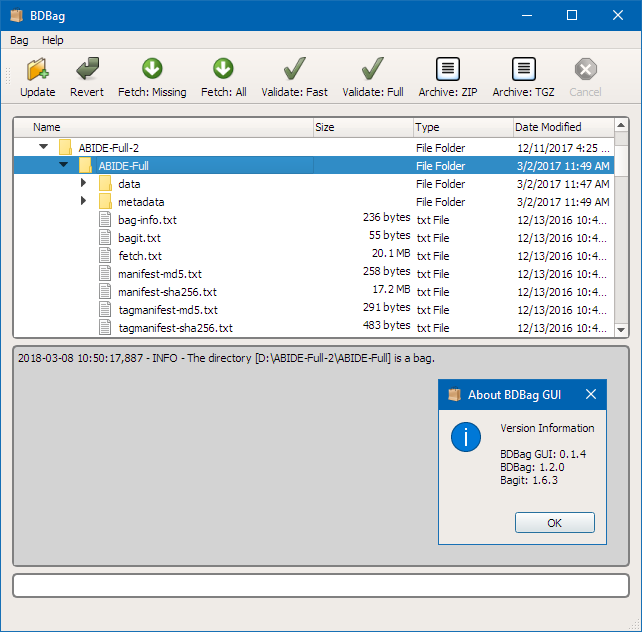
\includegraphics[width=0.49\textwidth]{figs/bdbag_gui_version.png}
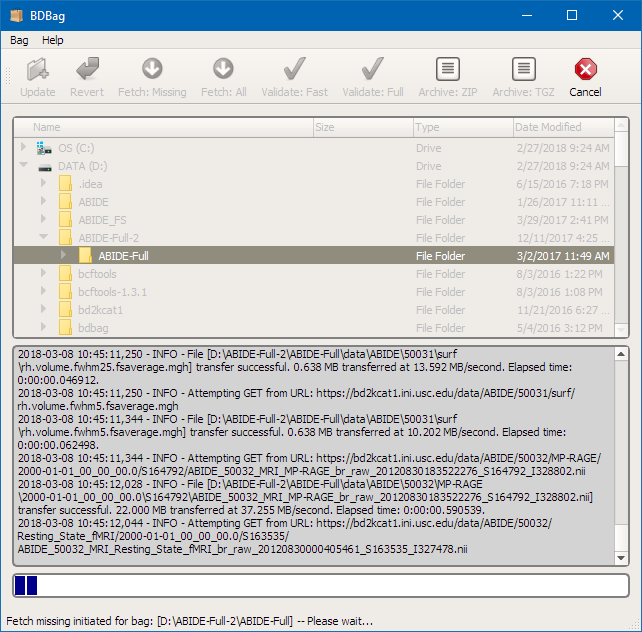
\includegraphics[width=0.49\textwidth]{figs/bdbag_gui_fetch.png}
\caption{Two views of the BDBag GUI. 
On the left, the user is browsing a BDBag named ABIDE-Full. The top pane shows the operations
supported. On the right, the user has initiated a ``Fetch Missing" operation on the ABIDE-Full
bag. Progress is shown in the lower panes.\label{fig:gui}}
\end{figure}



\subsection{Tools that use BDBag and Minid APIs}

We have developed a range of additional tools that provide useful functionality to users.
These tools also serve as examples of how to integrate BDBag and Minid
capabilities into applications.

\subsubsection{The \texttt{bagofbags} tool}

This application, which creates a bag that itself contains bags, is a nice example of how to
use BDBag and Minid APIs to create new capabilities.
It is used, for example, in the transcription factor
binding site study~\cite{madduri2018reproducible}.
See \smallurl{https://github.com/ini-bdds/bdbag/tree/master/examples/bagofbags}.
%Figure~\ref{fig:bob}, from the \texttt{bagofbags} documentation, illustrates its use.
%
%\begin{figure}
%\centering
%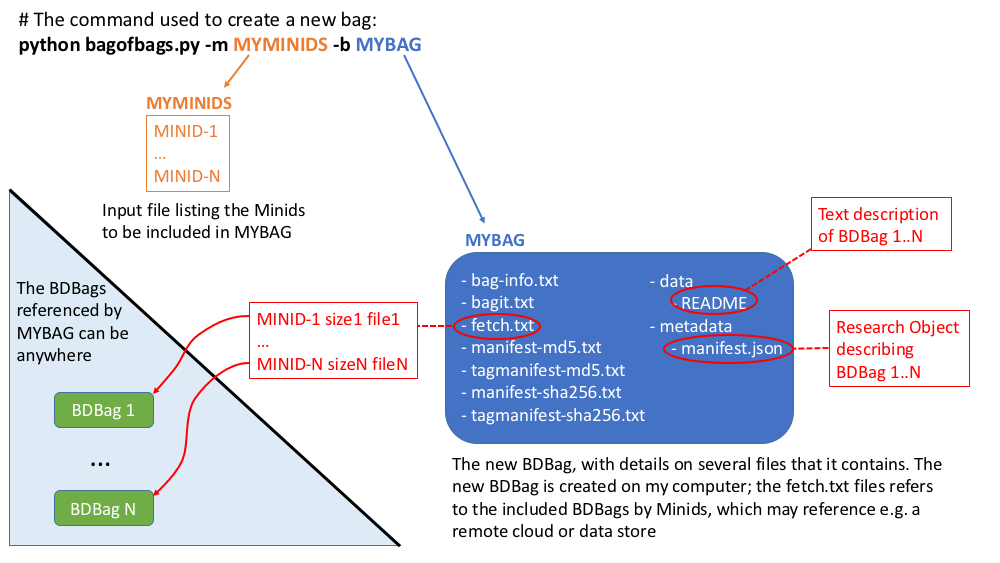
\includegraphics[width=0.8\textwidth]{figs/MetaBags.png}
%\caption{At top, an example use of the \texttt{bagofbags} tool; below, an illustration of the BDBag created, which contains the usual files that are to be found in a BDBag, with the \texttt{fetch.txt} file containing the Minids that can be used to fetch their contents and the \texttt{data/manifest.json} containing descriptive metadata. In addition, the \texttt{data/README} file contains background information.\label{fig:bob}}
%\end{figure}

\subsubsection{The Data Concierge services}

%This service takes a set of Search results, creates a BDBag, and tracks the location with a Minid.
The Concierge Services implement a set of REST APIs secured with Globus Auth that handle common patterns around data management, using standards wherever possible. 
The \texttt{search2bag} service accepts a set of URIs to datasets and returns a digital identifier (a Minid) that references a BDBag stored in a configurable location such as S3. 
This can be used to track groupings of datasets by users in a portal, for example, with the Minid acting as the primary key. 
The \texttt{stagebag} service can be incorporated into workflows to simplify data transfers and staging by users. 
It takes as parameters one or more Minids referencing BDBags plus
%on the assumption that the remote references for the data in the BDBags are Globus URIs. 
a destination Globus endpoint and path. 
%It iterates through the URIs referenced in the BDBags and submits a Globus Transfer request to the destination.
It initiates a Globus transfer request and returns the associated identifier so that  
 the portal or user can monitor its progress. 
%The final planned Service, \texttt{checkbag}, is in development. 
%It will utilize a remote checksum storage API to compare the checksums of files on an endpoint with those in the BDBag. 
%This enables the creation of integrity checking services, and also allows users to know which files they may have modified during their work.
See \smallurl{https://github.com/ini-bdds/data-concierge}.

\subsubsection{The \texttt{encode2bag} tool}

%We use a genomics example to illustrate how the BDBag and Minid tools can be used to reduce
%barriers to data sharing and reproducibility.
The 
%Encyclopedia of DNA Elements (ENCODE) 
ENCODE consortium 
%operates a database that aims to provide a
%comprehensive parts list of functional elements in the human genome.
ENCODE provides a web portal that a researcher can use to query its database,
using menus to specify parameters such as assay, biosample, and genomic annotations.
The result is a set of data URLs,
which must be downloaded individually and unfortunately do not come with associated metadata or context.
%Researchers often resort to building shell scripts to download and store the raw datasets.
These manual data retrieval and management steps can be error-prone,
time consuming, and difficult to reproduce.
%Researchers must manually save results to record data provenance (posing the same query to the database at different times may give different results)
%and the only way to validate that downloaded files have not been corrupted is to download them again.
%In other words, the ENCODE portal is not particularly supportive of FAIR research.

We thus used BDBag, Minid, and Globus tools to create a lightweight command line utility and web service, \texttt{encode2bag}.
A researcher % uses either the web interface or the command line interface to 
specify required data;
the service makes the data available,
%either enter an ENCODE query or upload an ENCODE metadata file describing a collection of datasets.
%They can then access the corresponding data, 
\emph{plus associated metadata and checksums}, as a BDBag.
%Selecting the ``Create BDBag'' button triggers the creation of a $\sim$100 kilobyte 
This BDBag encapsulates references to the files in question, metadata associated with those files, 
the query used to identify the data, and the checksums required to validate the files and metadata.
%The BDBag is stored in AWS Simple Storage Service (S3) cloud storage from where it can be accessed for purposes of sharing, reproducibility, or validation.
%Because this BDBag contains references to data, rather the data themselves, it captures the entire response to the query in a small (hundreds of kilobytes) form that can be easily downloaded, moved, and shared.
When needed, all, or a subset of, the files named within the BDBag's \texttt{fetch.txt} file can be downloaded
(using BDBag tools), while ensuring that their contents match those of the original query.
To further streamline access to query results, \texttt{encode2bag} assigns a Minid for each BDBag that it creates.
%so as to provide for unambiguous naming and identification of research data products for data provenance.
The Minid can be passed between services as a concise reference to the BDBag.

The \texttt{encode2bag} service and client side tool are available on GitHub at
\smallurl{https://github.com/ini-bdds/encode2bag} and 
\smallurl{https://github.com/ini-bdds/encode2bag-service}.

\vspace{2ex}

\noindent\shadowbox{%
    \parbox{0.985\textwidth}{%
The \texttt{encode2bag} service illustrates how BDDS BDBag and Minid tools
can be used to 
transform a clumsy, error-prone, and profoundly unFAIR process into one that is streamlined,
robust, and inherently FAIR, while simplifying the work of the researcher.
}}


\section{An Example Application}

BDBags and Minids proved vital when creating a reproducible version~\cite{madduri2018reproducible}
of a workflow developed by Funk et al.~\cite{funk18} to use ENCODE data to identify candidate
transcription factor binding sites. 
Funk et al.\ used \texttt{encode2bag} to create BDBags for each of 27 tissue types, each with its own Minid.
These 27 BDBags contain references to a total of 2.4 TB of ENCODE data;
references that can be followed at any time to access the associated data.
A separate BDBag (a ``bag of bags"), created with the \texttt{bagofbags} tool described earlier,
contains references to each of the 27 tissue type bags.

The transcription factor binding site application also demonstrates how BDBag and Minid mechanisms
can be integrated into other biomedical tools.
For example, the large parallel cloud computations used to process ENCODE data were all performed
with the Galaxy-based Globus Genomics.
We extended Globus Genomics so that when a workflow is passed, as an argument, a Minid 
that references a BDBag, 
the contents of that BDBag are retrieved and passed to the analysis workflow.
Figure~\ref{fig:5} shows the use of this capability.

\vspace{2ex}

\noindent\shadowbox{%
    \parbox{0.985\textwidth}{%
BDBags and Minids made it possible to capture all data consumed and produced by this complex,
computationally intensive, and distributed computation in a form that makes reproducibility and reuse
straightforward, whether by the authors as new data is obtained or by other researchers.
}}


\begin{figure}
\centering
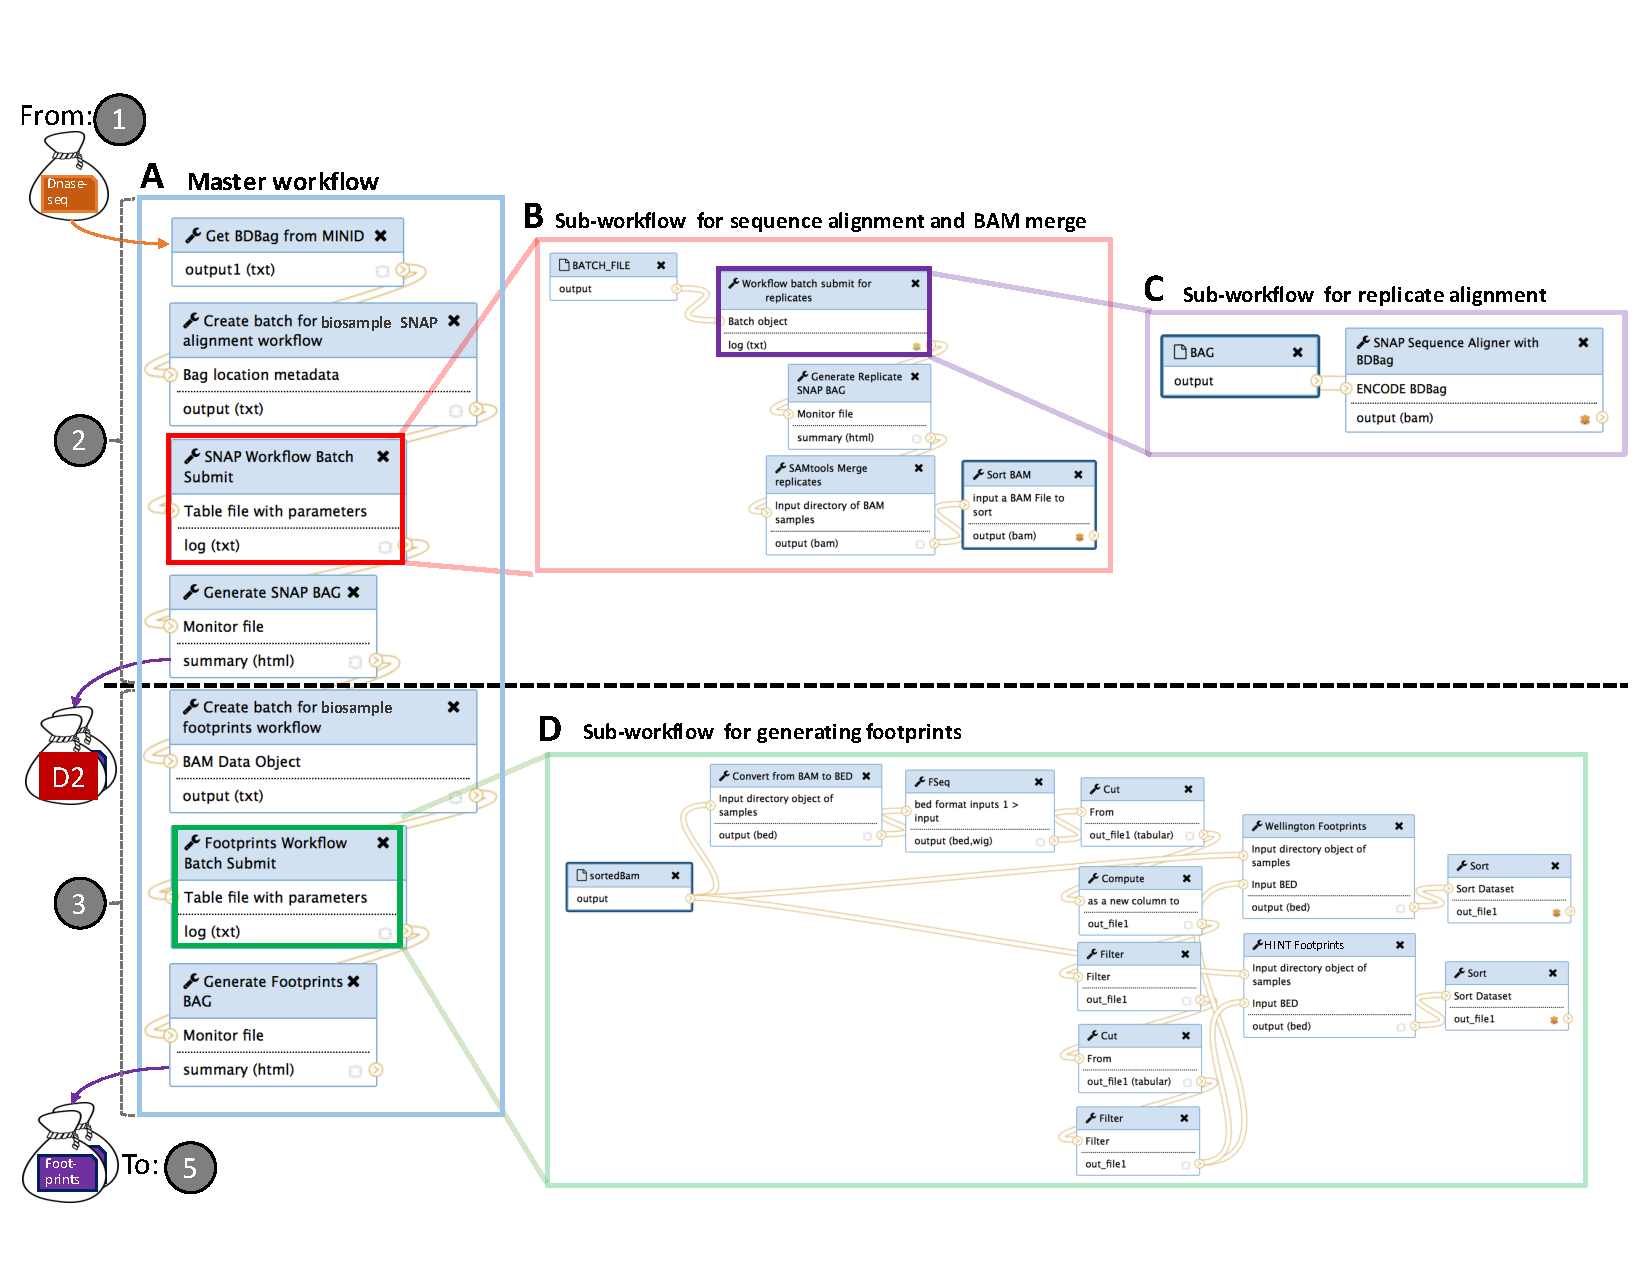
\includegraphics[width=0.8\textwidth,trim=0.1in 0.4in 0in 0.6in,clip]{figs/Fig4-02-20}
\caption{This figure, from Madduri et al.~\cite{madduri2018reproducible}, 
shows how BDBags (each designated by a Minid) are used to package inputs and outputs for the
 DNase-seq ensemble footprinting workflow of Funk et al.~\cite{funk18}.
\label{fig:5}}
\end{figure}


\section{External Impact}

GitHub provides us with some information about who is using our BDBag and Minid software,
in that we can search to see where the software is included in other public GitHub repositories. 
%This usage, plus the number who have ``starred" the BDBag repository, is a nice validation of the utility of the work. 
For example:

\begin{itemize}
\item
The BD2K BDDS project use BDBags and/or Minids in the following products: % developed within BDDS:

\vspace{-2ex}

\begin{itemize}
\item
Encode2Bag client and service: \smallurl{https://github.com/ini-bdds/encode2bag} and 
\smallurl{https://github.com/ini-bdds/encode2bag-service}

\item
SOCR-Dashboard: \smallurl{https://github.com/BD2K/SOCR-Dashboard}

\item
Peptide Atlas: \smallurl{http://www.peptideatlas.org/}
\end{itemize}

\item
BD2K BDDS team participants have also integrated BDBags and Minids into other tools 
developed in part with resources external to BDDS:

\vspace{-2ex}

\begin{itemize}
\item
The USC/ISI Discovery Environment for Relational Information and Versioned Assets (DERIVA) 
team uses BDBag and Minid for data import and export, enabling interoperability with other elements of the big biomedical data ecosystem. See \smallurl{http://isrd.isi.edu/deriva/} and \smallurl{https://github.com/informatics-isi-edu/deriva-py}.
\item
The UChicago team uses BDBags and Minids for data import and export within Globus Genomics 
(\smallurl{http://globusgenomics.org/}). See \smallurl{https://github.com/globusgenomics/genomics-footprint}.
\end{itemize}

\item
A number of groups external to BDDS are using BDBag and Minid technology in biomedical projects:

\vspace{-2ex}

\begin{itemize}
\item
The NIDCR-funded Facebase resource (see \smallurl{https://www.facebase.org}) uses DERIVA, and hence BDBags and Minids, for data import and export.

\item
The Galaxy project (\smallurl{https://galaxyproject.org/}) is integrating BDBag and Minid support for data import and export. 
See \smallurl{https://github.com/galaxyproject/galaxy}.

\item
The Gene Ontology (\smallurl{http://geneontology.org/}) project is integrating BDBag and Minid support for data import and export.
See \smallurl{https://github.com/geneontology}.

\item
The Monarch Initiative (\smallurl{https://monarchinitiative.org} is evaluating BDBags for data import and export. See
\smallurl{https://github.com/monarch-initiative/dipper/issues/551}.

\item
The NIH National Center for Advancing Translational Research (NCATS) Data Translator team
(https://ncats.nih.gov/translator) uses BDBags
in its ``smart bag" technology. See 
\smallurl{https://github.com/NCATS-Tangerine/smartBag}.

\item
The University of Chicago Center for Data Intensive Science (CDIS) is considering 
BDBag and Minid for use within its Peregrine/IndexD, as a basis for interoperability with other elements
of the NIH Data Commons. \smallurl{https://github.com/uc-cdis/indexd} and \smallurl{https://github.com/uc-cdis/peregrine}
\end{itemize}

\item
BDBags and Minids are also being used outside biomedicine. For example, they are being integrated
into the Materials Data Facility (\smallurl{https://www.materialsdata facility}) as a standard format for data import and
export. 

\end{itemize}

%\vspace{2ex}

\noindent\shadowbox{%
    \parbox{0.985\textwidth}{%
BDBags and Minids are also being evaluated as a common interoperability mechanism within the new NIH Data Commons Pilot Program (DCPP).  
To date, BDBags and Minids have been adopted by four of the DCPP ``full stack" projects, 
and are being evaluated for use by several additional teams.
}}


\small
\bibliographystyle{abbrv}
\bibliography{refs,minid}

\end{document}
